\documentclass[dvipdfmx]{jsarticle}
\usepackage{tikz}
\usepackage{amsmath}
\usepackage{amssymb}
\usepackage{amsfonts}
\usetikzlibrary{positioning}

\newcommand{\yslant}{0.4}
\newcommand{\xslant}{-0.6}

\begin{document}
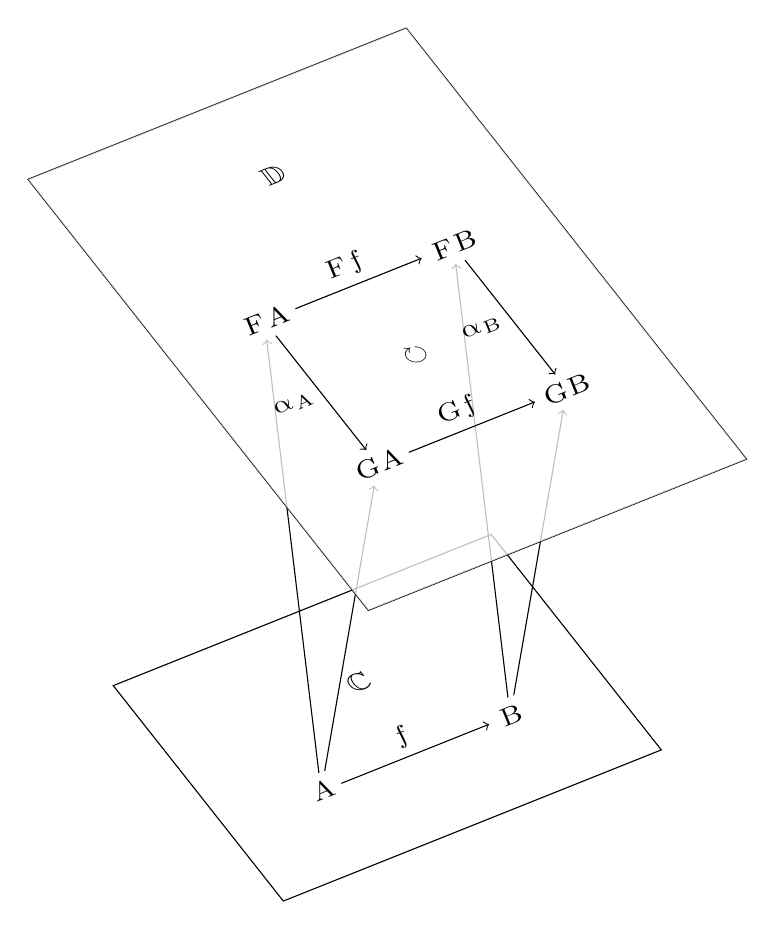
\begin{tikzpicture}[scale=1.2]
    \begin{scope}[yshift=-120, every node/.append style={yslant=\yslant,xslant=\xslant}, yslant=\yslant,xslant=\xslant]
        \draw (0,0) rectangle (4,3); % フレーム
        \node at (2, 2) {$\mathbb{C}$};
        \node (A) at (1, 1) {$A$};
        \node (B) at (3, 1) {$B$};

        \draw[->] (A) -- (B) node[midway, above] {$f$};
    \end{scope}
    
    \begin{scope}[yshift=0, every node/.append style={yslant=\yslant,xslant=\xslant}, yslant=\yslant,xslant=\xslant]
        \draw (0,-1.5) rectangle (4,4.5); % フレーム
        \node (FA) at (1, 2) {$FA$};
        \node (FB) at (3, 2) {$FB$};
        \node (GA) at (1, 0) {$GA$};
        \node (GB) at (3, 0) {$GB$};
    \end{scope}

    \draw[->] (A) -- (FA);
    \draw[->] (B) -- (FB);
    \draw[->] (A) -- (GA);
    \draw[->] (B) -- (GB);

    \begin{scope}[yshift=0, every node/.append style={yslant=\yslant,xslant=\xslant}, yslant=\yslant,xslant=\xslant]
        \draw[opacity=.75] (0,-1.5) rectangle (4,4.5); % フレーム
        \fill[white,opacity=.75] (0,-1.5) rectangle (4,4.5);
        \node at (2, 3.5) {$\mathbb{D}$};
        \node (FA') at (1, 2) {$FA$};
        \node (FB') at (3, 2) {$FB$};
        \node (GA') at (1, 0) {$GA$};
        \node (GB') at (3, 0) {$GB$};
        
        \draw (2,1) node{$\circlearrowright$};

        \draw[->] (FA') -- (FB') node[midway, above] {$F f$};
        \draw[->] (GA') -- (GB') node[midway, above] {$G f$};
        \draw[->] (FA') -- (GA') node[midway, left] {$\alpha_A$};
        \draw[->] (FB') -- (GB') node[midway, left] {$\alpha_B$};
    \end{scope}


\end{tikzpicture}
\end{document}
